The \stview visualizes a \stree, which was generated as described in 
\subsecref{sec:scaffoldhunter:treegeneration}. 

\subsection{Navigation}
A new \stview will show an overview of the whole graph. You may zoom in to get
more detailed information on a part of the graph. Depending on the scale,
scaffolds will be represented simplified by a rectangle or by their structural
formula. There are several ways to zoom in/out: You may use the mouse wheel to
magnify/demagnify the view on the area of the mouse pointer or by using the
buttons in the \tbar or \gui{Tree} menu. You may also select the area of
interest by a rectangle on the GraphMap, see
\subsecref{sec:treeview:graphmap}. The other navigation mechanism is
panning: By keeping the left mouse button pressed on an empty area in the graph
pane and moving the mouse the viewpoint is panned. You may also use the
scrollbars for panning.

Usually not all scaffolds are shown when a new \stview is opened. Subtrees
beginning at a scaffold can be shown or hidden respectively by clicking on the
+/-- symbol at the lower left corner of the scaffold. In addition, the context menu
(\subsecref{sec:treeview:contextmenu}) contains options to open complete
subtrees or to open all children on the next hierarchy level. Inverse operations
exist to hide scaffolds you are not interested in. The command to expand the
whole tree or to reset it to the default hierarchy level can be invoked via the
\tbar or  \gui{Tree} menu (\subsecref{sec:treeview:menutoolbar}).

A scaffold will be shown in different colors based on the global selection as
described in \subsecref{sec:linking:selection}. A left-click on an unselected or
partially selected scaffold will add all molecules associated with the scaffold
to the selection, a left-click on a fully selected scaffold will deselect all
associated molecules.

You may also navigate using keyboard shortcuts, listed in
\appref{chap:scaffoldhunter:shortcuts}. There is a cursor set on one scaffold
marked by a blue rectangle. The cursor can be  moved using the arrow keys. The
camera automatically retains focus on the cursor.


\subsubsection{GraphMap} \label{sec:treeview:graphmap}
The GraphMap is found in the \sbar on the left hand side and provides an
overview on the whole graph. The current viewport of the graph pane is marked by
a transparent red rectangle. Dragging this rectangle with the mouse will change
the viewport of the graph pane accordingly. Click the left mouse button at an
area that is not currently visible to center the viewport on the selected point.
You can define a new viewport by marking a rectangle on the graph map: Click the
left mouse button on an empty area and keep it pressed while moving the mouse.
When releasing the mouse button the view will be panned and zoomed to completely
contain the selected area. Using your mouse wheel on the GraphMap will magnify
or demagnify the graph pane at the specified point.

\subsubsection{Magnifying Glass}
The Magnifying Glass in the \sbar below the GraphMap is opened by a mouse click on its title bar. It shows the area below the mouse 
pointer magnified. You may move the mouse pointer over the graph pane and navigate in the graph as usual while the Magnifying Glass is 
active.



\subsection{Context Menu} \label{sec:treeview:contextmenu}
\begin{figure}[!htb]
   \centering
   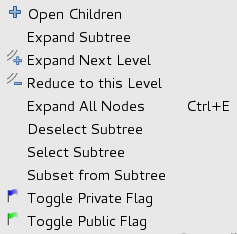
\includegraphics[width=0.3\textwidth]{images/stree/contextmenu.png}
   \caption[\Stview contex menu]{The context menu invoked by a right-click on a scaffold.}
   \label{fig:scaffoldhunter:contextmenu}
\end{figure}
Click the right mouse button on a scaffold to access the context menu. The menu mainly contains options that are directly related to the 
scaffold: You can open/close the children of the scaffold, open the whole subtree rooted at the scaffold or open all children on the next 
hierarchy level by the option \gui{Expand next level}. In addition you can
choose to expand the whole tree, by clicking on \gui{Expand all Nodes}. You can
hide the hierarchy levels under the scaffold by choosing \gui{Reduce to this
level}.

The commands \gui{Select Subtree} and \gui{Deselect Subtree} add or remove all
molecules from the selection, which are associated with scaffolds located in the
subtree that is rooted at the current scaffold. The command \gui{Subset from
Subtree} will create a new subset which contains these molecules.

There are two additional entries to set or remove public and private flags, see
\subsecref{sec:linking:flags}.

\subsection{Tree Menu \& Tool Bar} \label{sec:treeview:menutoolbar}
\begin{figure}[!htb]
   \centering
   
\includegraphics[width=0.9\textwidth]{images/stree/toolbar.png}
   \caption[\Stview \tbar]{
      Meaning of the icons (from left to right): Zoom In, Zoom Out, Fit Graph,
      Fit Selection, Expand all Nodes, Number of Rings to Default Level,
      Increase/Decrease Radius, Lock Radii while Zooming, Scale cusor node
      up/down, Normalize cursor node, Scale Selected Scaffolds up/down,
      Normalize Selected Scaffolds, Normalize all Scaffolds, Configure Property
      Mappings, Show Scaffold Molecules, Export Image
   }
   \label{fig:treeview:toolbar}
\end{figure}

The \gui{Tree} menu provides access to many different functions related to the
\stview. The \tbar shown in \shortfigref{fig:treeview:toolbar} allows quick
access to most of these functions. When you hover the cursor over an item of the
menu or \tbar a tooltip with a description will appear. It follows a list of
the menu items, each with a short description.

\begin{description}
 \item [Layout] Can be used to choose one of the three available layout algorithms. The graph in the current tab will be laid out accordingly. 
See \subsecref{sec:treeview:layout} for a brief description of the layouts.
 \item [Show Scaffold Molecules] Toggles the molecule view for each node in the
 scaffold tree, which displays the molecules associated with a scaffold.
 \item [Configure Property Mappings] Allows to map different imported
 properties to several visual features of the nodes in the \stree{}. See
 \subsecref{sec:treeview:propertymappings} for details.
 \item [Zoom In/Out] Changes the zoom level of the graph pane.
 \item [Fit Graph] Changes the zoom level and pans the graph pane to show the
 whole graph.
 \item [Fit Selection] Changes the zoom level to show all selected and partially
 selected scaffolds.
 \item [Expand all Nodes] Expands the whole Graph.
 \item [Number of Rings to Default Level] Resets the graph, such that only the
 hierarchy levels which are shown by default are displayed.
 \item [Increase/Decrease Radius] Allows adjustment of the distance between two
 adjacent rings in the radial layout.
 \item [Lock Radii While Zooming] Disables/enables the automatic adjustment of the distance
 between two adjacent rings in the radial layout.
 \item [Node Scale] Resizes the scaffolds of the graph. There are buttons for
 scaling up/down all currently selected scaffolds or just the scaffold the
 cursor is on. In addition \gui{Normalize} buttons are provided to reset
 scaffolds to their original size.
 \item [Export Image] Allows exporting the current viewport or the whole graph
 as an image. 
\end{description}

\subsection{Layout} \label{sec:treeview:layout}
\begin{figure}[!htb]
   \centering
   \subfloat[][] {
      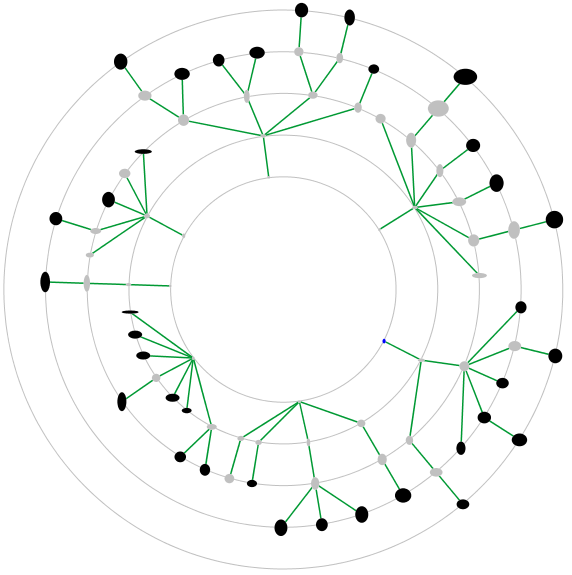
\includegraphics[scale=0.3]{images/stree/sh_layout_radial.png}
      \label{fig:treeview:layout:radial}
   }
   \quad
   \subfloat[][] {
      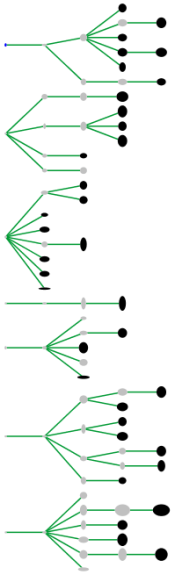
\includegraphics[scale=0.3]{images/stree/sh_layout_linear.png}
      \label{fig:treeview:layout:linear}
   }
   \quad
   \subfloat[][] {
      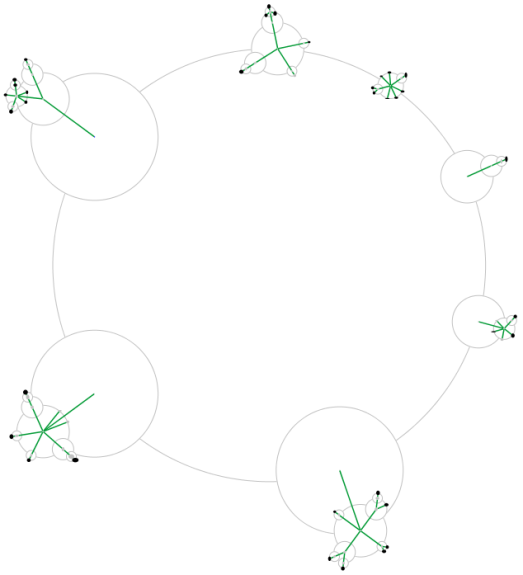
\includegraphics[scale=0.3]{images/stree/sh_layout_balloon.png}
      \label{fig:treeview:layout:balloon}
   }
   \caption[\Stview layouts]{
      Different layouts of the same graph: \subref{fig:treeview:layout:radial} Radial Layout, \subref{fig:treeview:layout:linear} Linear Layout, \subref{fig:treeview:layout:balloon} Balloon Layout
   }
   \label{fig:treeview:layout}
\end{figure}
\sh offers three different layouts, which can be selected by using the
\gui{Layout} option in the \gui{Tree} menu \subsecref{sec:treeview:menutoolbar}.
The different layouts are shown in \shortfigref{fig:treeview:layout}. The Radial Layout
(\shortfigref{fig:treeview:layout:radial}) is the default layout method. 
With this layout the scaffolds are located according to their depth on circles
with a common center. The Linear Layout (\shortfigref{fig:treeview:layout:linear}) orders the
scaffolds from left to right. Both layouts emphasize the depth of scaffolds.
With the Balloon Layout (\shortfigref{fig:treeview:layout:balloon}) each scaffold is the
center of a circle on which its children are distributed. This 
layout separates subtrees more clearly from each other.

For the Radial Layout the distance between the circles may be customized. By default the
distance is automatically adjusted depending on the zoom. The \gui{Lock Radii
While Zooming} button disables this mechanism and allows the user to set the
distance using the buttons \gui{Increase Radius}/\gui{Decrease Radius}.

\subsection{Sorting}
Initially the ordering of scaffolds in the tree is chosen in a deterministic
way but without any meaning. Alternatively scaffolds can be sorted according to
some property value using the \gui{Sort} \sbar panel
show in \shortfigref{fig:treeview:sortpanel}.

The same panel can be used to define the ordering of the molecules which are
shown when the option \gui{Show Scaffold Molecules} is toggled. To do so select
the property by which these molecules should be sorted in the uppermost box.

\begin{figure}[!htb]
   \centering
   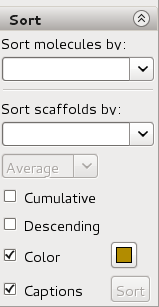
\includegraphics[scale=0.5]{images/stree/sidebar_sort.png}
   \caption{The Sidebar sort panel}
   \label{fig:treeview:sortpanel}
\end{figure}
The property used for sorting can be chosen using the box below \gui{Sort
Scaffolds by}. An accumulation method to determine how scaffold
properties will be derived from the properties of associated molecules can be selected in the
box below. The checkboxes underneath can be used to add a colored background to
the graph, where each segment which has the same value of the selected property
is colored in the same shade of the selected color. A label showing this value
can be displayed in each segment.

After clicking on \gui{Sort} the scaffolds on the first layer will be reordered
according to their property values. Sorting by property values is applied only
to the scaffolds on the first layer. You can however create a subset out of a
subtree and sort the \stree displaying the subset. 

\subsection{Property Mappings}
\label{sec:treeview:propertymappings}
Properties associated with the scaffolds can be mapped to different \emph{visual
properties} of the Scaffold Tree. Scaffold properties are either directly
associated with a scaffold, such as \emph{Number of Oxygen Atoms} or can be
derived from the properties of the structures  which are associated with a
scaffold.

The following \emph{visual properties} are available for mapping:

\paragraph{Node Background Color} This changes the background color of the
scaffold nodes in the scaffold tree. Either two colors can be selected and the
value range of the property is mapped to the gradient between those two colors
or value intervals can be specified and a color can be assigned to each
interval.

\paragraph{Edge Thickness} This maps the absolute difference between the values
associated with two adjacent scaffolds onto their connecting edge. The maximum
and minimum displayed thickness are predefined and cannot be adjusted. A
gradient mapping maps the greatest difference to the maximum thickness and the
smallest difference to the minimum thickness, intermediate differences are linearly
mapped to intermediate thickness values. Alternatively intervals of differences
can be defined, which will then be mapped to different thickness values.

\paragraph{Edge Color} Similarly to the way values can be mapped to the
background color of a node they can also be mapped to the adjacent edges. On the
edge a gradient between the colors will be displayed, which is determined by the
adjacent scaffolds.

\paragraph{Label} The value associated with a scaffold can be displayed by a
label below the node in the scaffold tree. 

\begin{figure}[h]
\centering
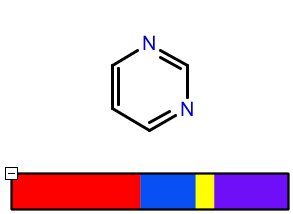
\includegraphics[scale=0.5]{images/stree/infobar.png}
\caption{An example of an Info Bar.}
\label{fig:treeview:infobar}
\end{figure}

\paragraph{Info Bar} This visualizes distributions of a property for the
molecules associated with a scaffold. Intervals can be specified and a
color is associated with each interval. The distribution of these intervals can then
be visualized as shown in \shortfigref{fig:treeview:infobar}. Textual properties
with ten different values or less can also be mapped to colors to display such a
distribution.

\begin{figure}[p]
\centering
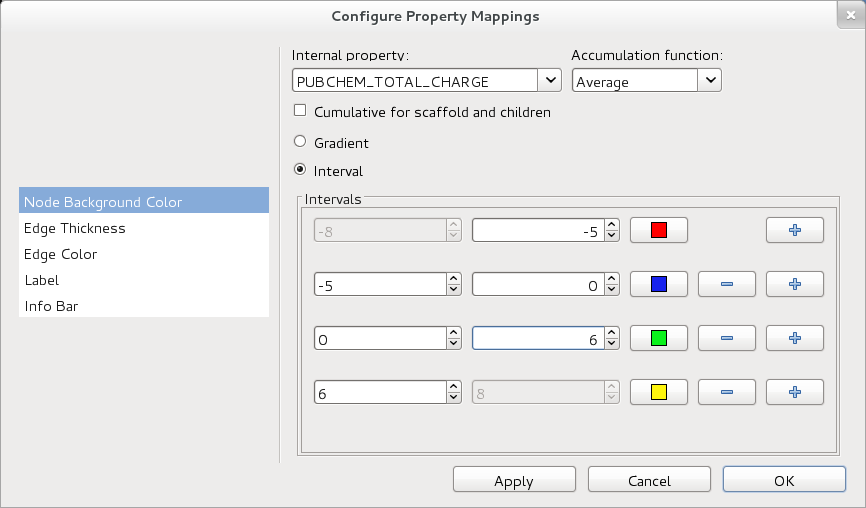
\includegraphics[scale=0.5]{images/stree/mappingdialog.png}
\caption{The property mapping dialog showing an interval mapping to the Node
Background Color.}
\label{fig:treeview:propmapdialog}
\end{figure}

The dialog to configure these mappings is shown in
\shortfigref{fig:treeview:propmapdialog}. On the left the visual property can be
selected, on the right settings for the selected visual property can be
configured. These settings may vary depending on the visual property. In general
the scaffold property to be mapped can be selected using the box at the top, in
case of \emph{derived properties} a second box will be displayed to select the
accumulation function. If the box \gui{Cumulative for scaffolds and children} below
is selected the accumulation function will not only be applied to values of
the structures associated with the scaffold, but also include the
values of all structures, which belong to scaffolds located in the subtree below
the scaffold.

\subsection{Exporting Images}
\label{sec:treeview:imageexport}

\begin{figure}[p]
\centering
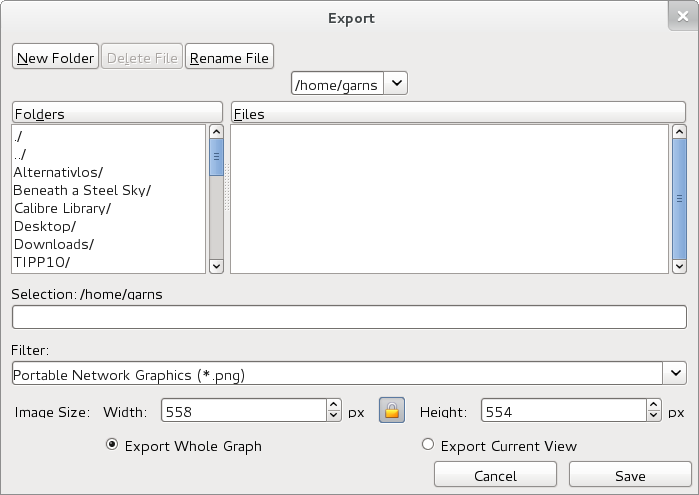
\includegraphics[scale=0.5]{images/stree/export.png}
\caption{The export dialog.}
\label{fig:treeview:export}
\end{figure}
Clicking the \gui{Export Image} button in the \tbar or the \gui{Tree} menu
will open the export dialog shown in \shortfigref{fig:treeview:export}, which
allows you to save the current graph as an image. You can either  export the
current view on the graph, which will save only the part of the graph
which is currently visible in the graph pane, or the whole graph. There are
three file formats available (SVG, PNG and TIFF) and options to control the
image size. By default the aspect ratio of the exported image is fixed, this can
be changed by clicking on the lock.

Since SVG is a file format for vector graphics the exported image can
be scaled without quality loss. Consequently the specified image size will not
have much effect on the quality or file size for SVGs but is very important for
raster formats such as PNG and TIFF. Even if the current view shows rectangles
for scaffolds the exported image will always show their structural formulas. 

\newpage
